\documentclass{article}

\usepackage{graphicx}
\usepackage{tikz}
\usepackage{tikzsymbols}
\usetikzlibrary{calc,patterns,shapes.geometric}
\pagestyle{empty}
\usepackage[margin=0pt]{geometry}
\geometry{papersize={14in,12in}}

\def\centerarc[#1](#2)(#3:#4:#5){\draw[#1] ($(#2)+({#5*cos(#3)},{#5*sin(#3)})$) arc (#3:#4:#5);}

\begin{document}
	\begin{figure}
		\centering
		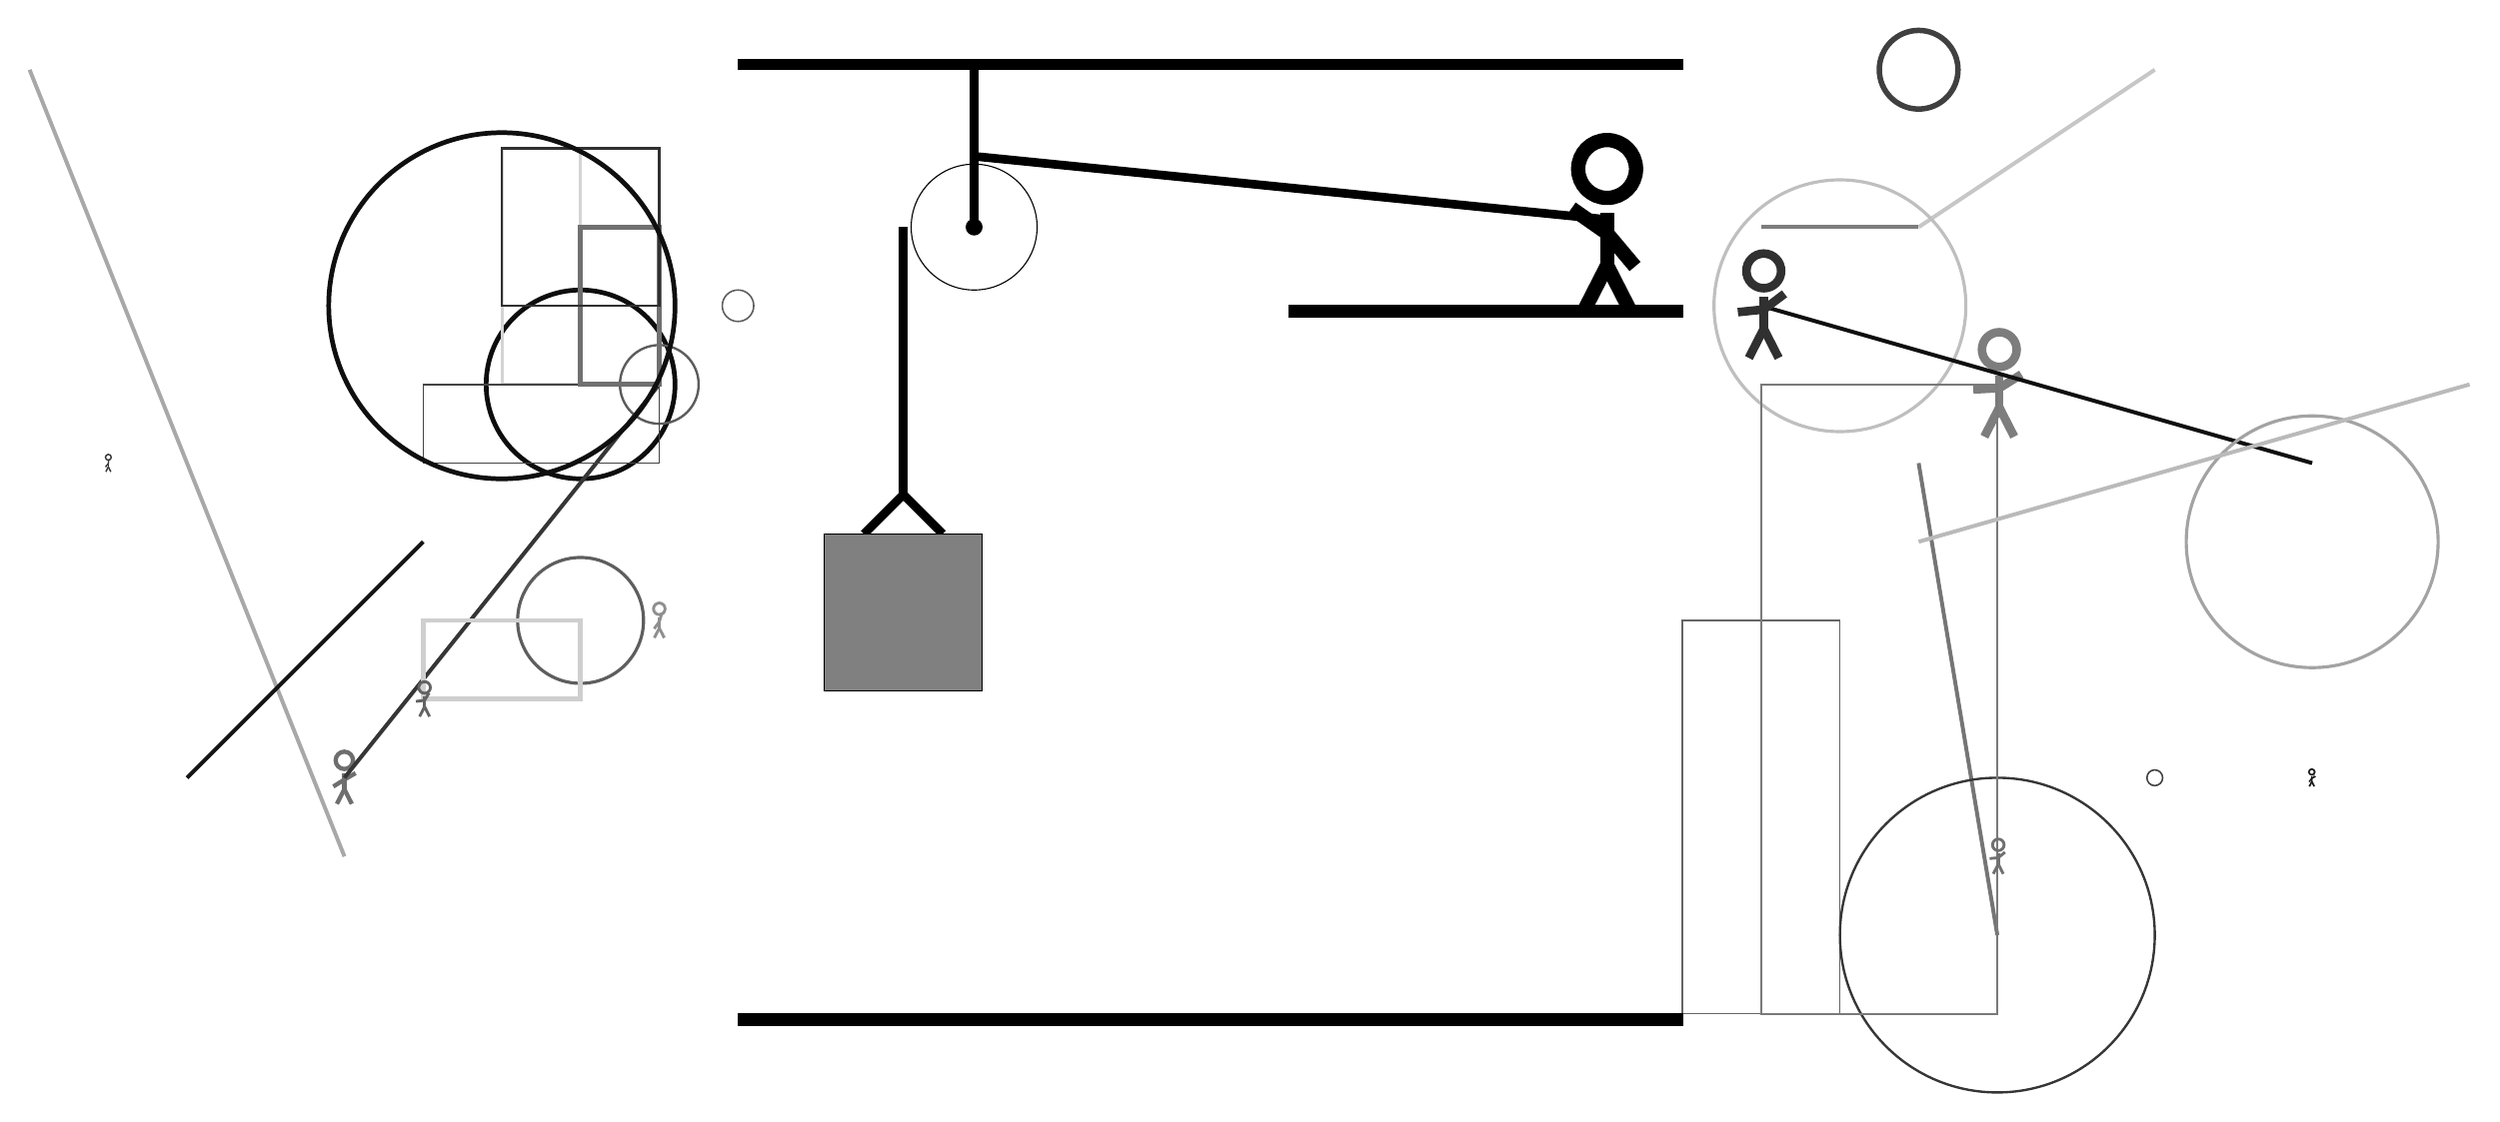
\begin{tikzpicture}
			%%%%% START %%%%%
			
			\draw[fill=black] (-2, 9) rectangle (10, 9.125);
			
			\draw (1, 7) circle (0.8);
			\draw[fill=black] (1, 7) circle (0.1);
			\draw[line width=1.1mm] (1, 9) -- (1, 7);
			
			\draw[line width=1.1mm](-0.4, 3.1) --  (0.1, 3.6) -- (0.6, 3.1);
			\draw[fill=black!50] (-0.9, 3.1) rectangle (1.1, 1.1);
			
			\draw[line width=1.1mm](0.1, 7) -- (0.1, 3.6);
			\centerarc[line width=1.1mm](1, 7)(90:180:0.9)
			\draw[line width=1.1mm](1, 7.9) -- (9, 7.1);
			
			\draw [line width=0.2mm, color=black!74](16, 0) circle (0.1);
			
			\draw [line width=0.6mm, color=black!95](-4, 5) circle (1.2);
			\draw [line width=0.3mm, color=black!64](-3, 5) circle (0.5);
			\draw [line width=0.4mm, color=black!63](-4, 2) circle (0.8);
			
			\draw[line width=0.5mm, color=black!54](13, 4) -- (14, -2);
			\node[line width=0.6mm, color=black!78] at (-10, 4) {\Strichmaxerl[1][48][86]};
			
			\node[line width=0.6mm, color=black!57] at (-7, 0) {\Strichmaxerl[3][32][30]};
			\draw[line width=0.4mm, color=black!17] (-4, 8) rectangle (-5, 5);
			\draw[line width=0.5mm, color=black!79](-7, 0) -- (-3, 5);
			\draw[line width=0.5mm, color=black!22](13, 7) -- (16, 9);
			\draw[line width=0.2mm, color=black!60] (12, 2) rectangle (10, -3);
			\draw[line width=0.5mm, color=black!34](-7, -1) -- (-11, 9);
			\draw[line width=0.6mm, color=black!19] (-4, 2) rectangle (-6, 1);
			
			\draw[line width=0.2mm, color=black!73] (-3, 4) rectangle (-6, 5);
			\node[line width=0.4mm, color=black!51] at (14, 5) {\Strichmaxerl[6][3][32]};
			\draw [line width=0.2mm, color=black!74](-11, 3) circle (0.0);
			\draw[line width=0.6mm, color=black!56] (-3, 5) rectangle (-4, 7);
			
			\draw [line width=0.4mm, color=black!25](12, 6) circle (1.6);
			\draw [line width=0.3mm, color=black!79](14, -2) circle (2.0);
			
			\draw[line width=0.3mm, color=black!81] (-3, 8) rectangle (-5, 6);
			\node[line width=0.4mm, color=black!45] at (18, 0) {\Strichmaxerl[1][85][56]};
			
			\draw[line width=0.5mm, color=black!94](11, 6) -- (18, 4);
			\draw[line width=0.5mm, color=black!51](13, 7) -- (11, 7);
			\draw[line width=0.3mm, color=black!52] (11, 5) rectangle (14, -3);
			\draw [line width=0.4mm, color=black!36](18, 3) circle (1.6);
			
			\draw [line width=0.2mm, color=black!63](-2, 6) circle (0.2);
			\draw[line width=0.5mm, color=black!92](-6, 3) -- (-9, 0);
			\draw [line width=0.6mm, color=black!94](-5, 6) circle (2.2);
			
			\node[line width=0.4mm, color=black!91] at (18, 0) {\Strichmaxerl[1][53][26]};
			\draw [line width=0.7mm, color=black!75](13, 9) circle (0.5);
			\node[line width=0.3mm, color=black!44] at (-3, 2) {\Strichmaxerl[2][54][73]};
			\node[line width=0.6mm, color=black!56] at (14, -1) {\Strichmaxerl[2][6][39]};
			\draw[line width=0.5mm, color=black!27](13, 3) -- (20, 5);
			
			\node[line width=0.2mm, color=black!81] at (11, 6) {\Strichmaxerl[6][6][37]};
			\node[line width=0.5mm, color=black!61] at (-6, 1) {\Strichmaxerl[2][7][59]};
			
			\node at (9, 7) {\Strichmaxerl[10][-35][-50]};
			\draw[fill=black] (5, 6) rectangle (10, 5.85);
			
			\draw[fill=black] (-2, -3) rectangle (10, -3.15);
			
			%%%%% END %%%%%
		\end{tikzpicture}
	\end{figure}	
\end{document}